\pdfoutput=1
\documentclass[a0,portrait,25pt]{sciposter}

% Служи за оформяне на текста в колони.
\usepackage{multicol}

% Задава разстоянието между колоните в постера.
\columnsep=20pt

% Задава дебелината на линията разделяща колоните в постера.
\columnseprule=1pt

% Задава цветове според техните SVG названия. Пълният списък с цветовете е наличен на: http://www.latextemplates.com/svgnames-colors
\usepackage[svgnames]{xcolor}

% Използване на Times шрифтовете.
\usepackage{times}

% Използва се за включването на изображения.
\usepackage{graphicx}
\graphicspath{{images/}}

% Позволява промяна на фоновия цвят. 
\usepackage{pagecolor}

% Позволява използването на текст в кутии и фонов цвят.
\usepackage{mdframed}

\begin{document}

% Фонов цвят на постера.
\pagecolor{LightGray}

\begin{mdframed}[backgroundcolor=white,roundcorner=4pt,shadow=true,linewidth=1pt]
\begin{minipage}[b]{1.44  \linewidth}
\begin{multicols}{2}
\
\color{DimGray}
\Huge \textbf{Sound Vectorization with Genetic Algorithms} \\
% Имена на авторите.
\huge {Petar Tomov, Iliyan Zankinski, Todor Balabanov} \\ [0.5cm] 
% Название на института.
\huge Institute of Information and Communication Technologies \\  Bulgarian Academy of Sciences \\ [0.4cm]
% Електронен адрес за връзка.
\Large \texttt{todorb@iinf.bas.bg}


\includegraphics[width=20cm]{logo-iict-en}
\end{multicols}
\end{minipage}
\end{mdframed}

% Разстояние между заглавната част на постера и същинското изложение. 
\vspace{0.5cm}

% Въведение. 
\begin{mdframed}[backgroundcolor=white,roundcorner=4pt,shadow=true,linewidth=1pt]
\color{Black}
\section*{Introduction}
In the audio based multimedia there are two common directions - WAVE audio and MIDI audio. The WAVE audio represents direct air vibrations assembled into a complex sound. On the other side MIDI audio is a sequence of musical events stating the order in which different musical notes should be played by different musical instruments. 
\end{mdframed}

% Разделя постера в три колони.
\begin{multicols}{3}

\begin{mdframed}[backgroundcolor=white,roundcorner=4pt,shadow=true,linewidth=1pt]
\color{Black}
\section*{Sound File Formats}
WAVE is a raw sound format and MIDI is a form of vector sound format. MIDI audio was developed with the progress of electronic musical instruments. It is an information representation standard which is very useful for real time audio information exchange and efficient file storage. 
\end{mdframed}

\begin{mdframed}[backgroundcolor=white,roundcorner=4pt,shadow=true,linewidth=1pt]
\color{Black}
\section*{Problem Definition}
To transform MIDI to WAVE is an easy task for the modern computers. It is done even inside the hardware sound cards by the module called MIDI synthesizer. The opposite transformation from WAVE to MIDI is relatively complex problem even for the modern computers. It is like a human that listens to the music and writing the notes corresponding to it. 
\end{mdframed}
 
\begin{mdframed}[backgroundcolor=white,roundcorner=4pt,shadow=true,linewidth=1pt]
\section*{Digital Ear \textregistered}
\begin{minipage}[c]{1\linewidth}
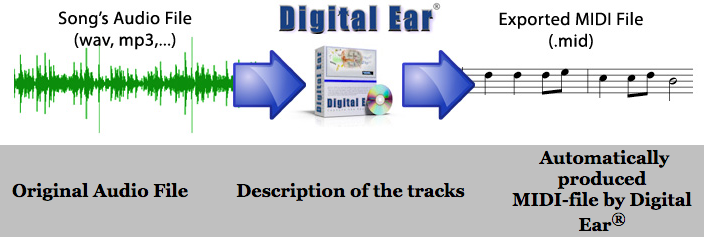
\includegraphics[width=1.0\linewidth]{pic002}
\end{minipage}
\end{mdframed} 

\begin{mdframed}[backgroundcolor=white,roundcorner=4pt,shadow=true,linewidth=1pt]
\color{Black}
\section*{Application of Vector Sounds}
Some audio information is not needed in WAVE or MP3 form but in MIDI (such as games background music). In these situations the WAVE information should be transformed in a group of simple MIDI events. This process of sound data transformation is related to information reduction. The process is transformation of true sounds into a set of simple musical events. 
\end{mdframed}
 
\begin{mdframed}[backgroundcolor=white,roundcorner=4pt,shadow=true,linewidth=1pt]
\section*{Mona Lisa}
\begin{minipage}[c]{1\linewidth}
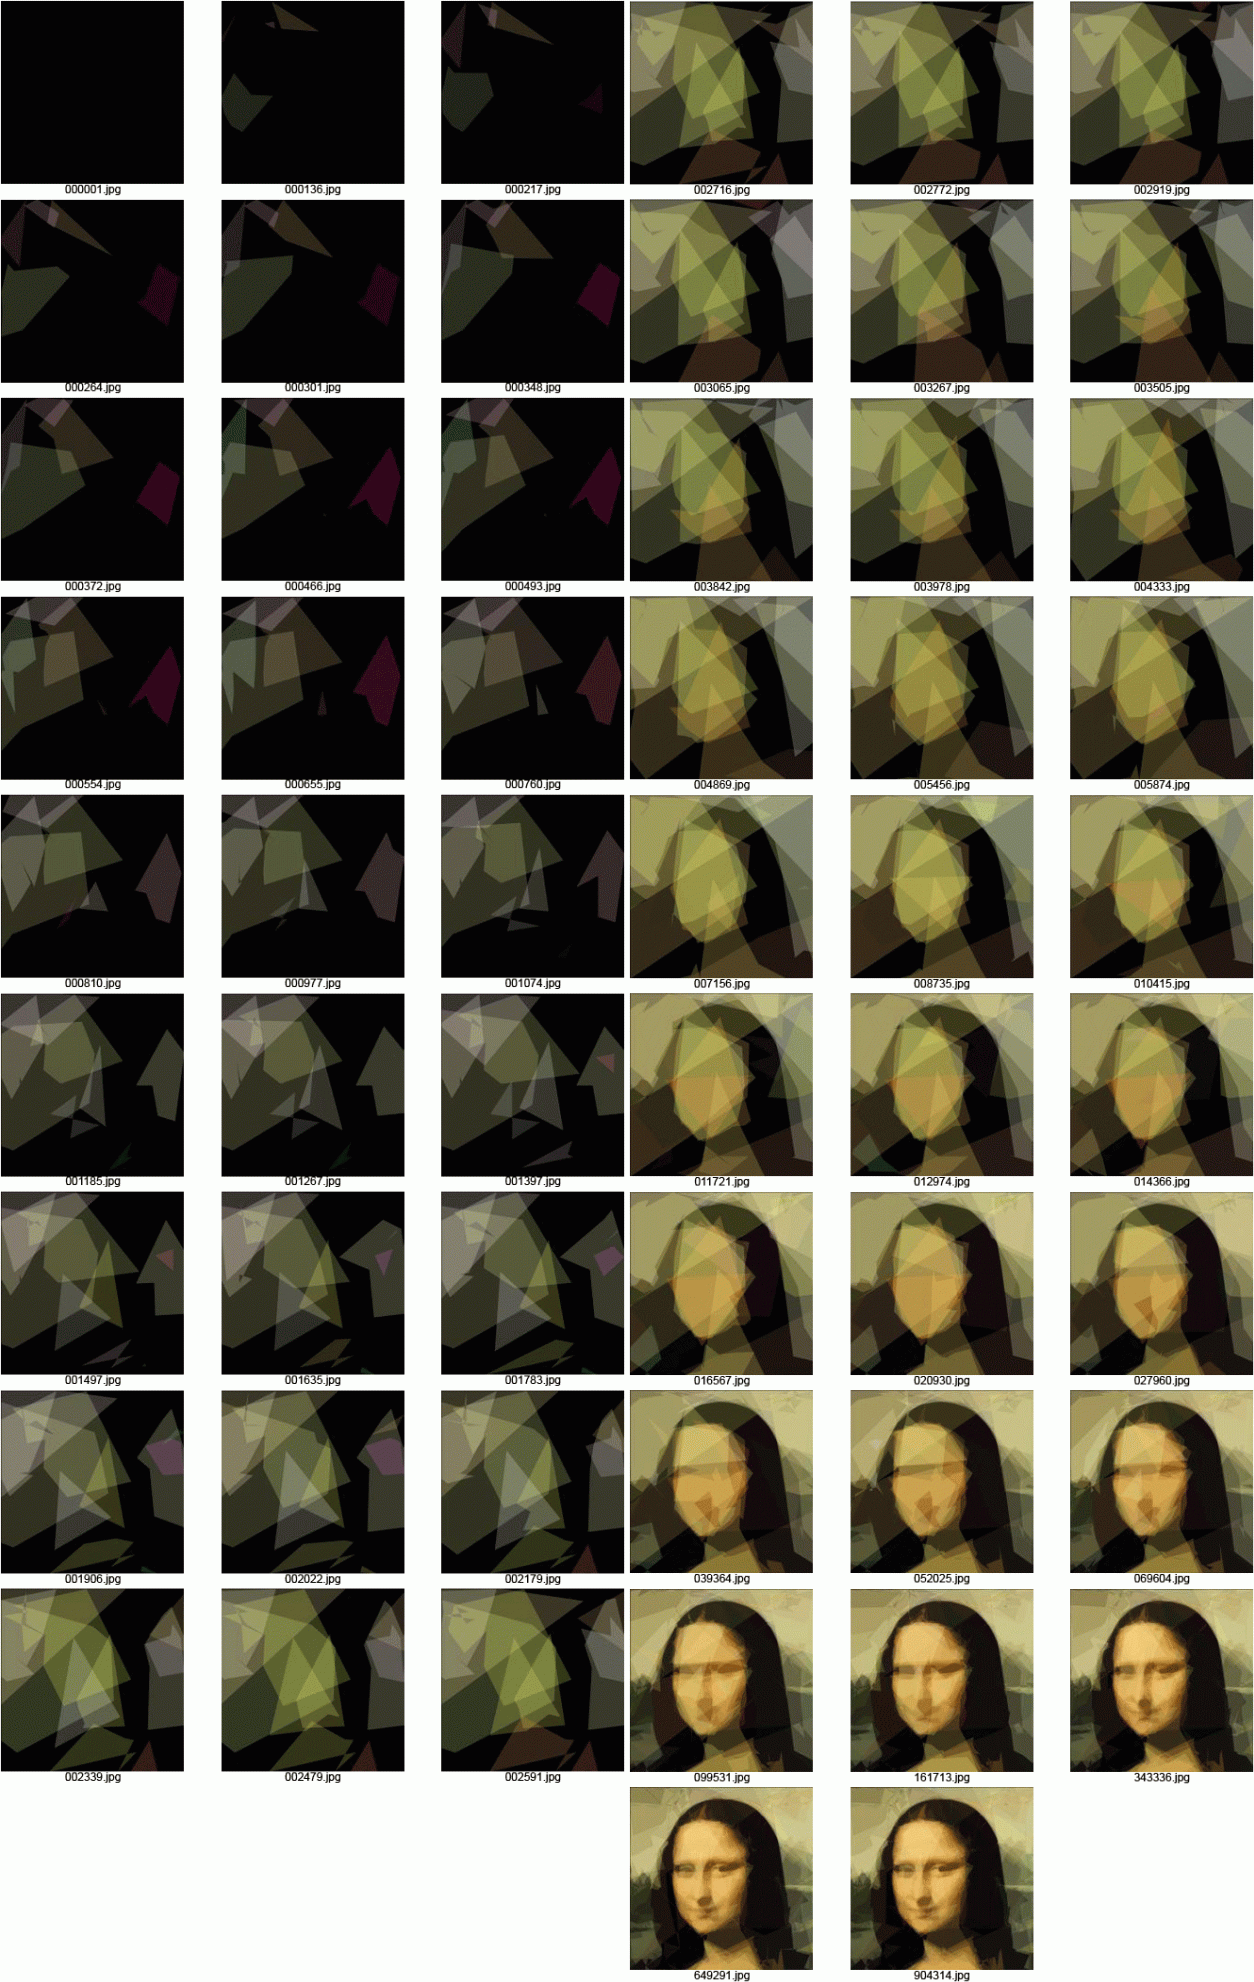
\includegraphics[width=1.0\linewidth]{pic001}
\end{minipage}
\end{mdframed} 

\begin{mdframed}[backgroundcolor=white,roundcorner=4pt,shadow=true,linewidth=1pt]
\color{Black}
\section*{Vectorization Analogies}
The problem of vectorization is very well known in literature and one of the most impressive implementations has been done with the image of Mona Lisa. The goal of this project was to approximate the picture of Mona Lisa by no more than 50 polygons. The colors and the points of the polygons were optimized with GAs. The same principles can be applied in sounds vectorization where WAVE information is transformed into a MIDI sequence.
\end{mdframed}

\begin{mdframed}[backgroundcolor=white,roundcorner=4pt,shadow=true,linewidth=1pt]
\section*{Genetic Algorithms}
\begin{minipage}[c]{1\linewidth}
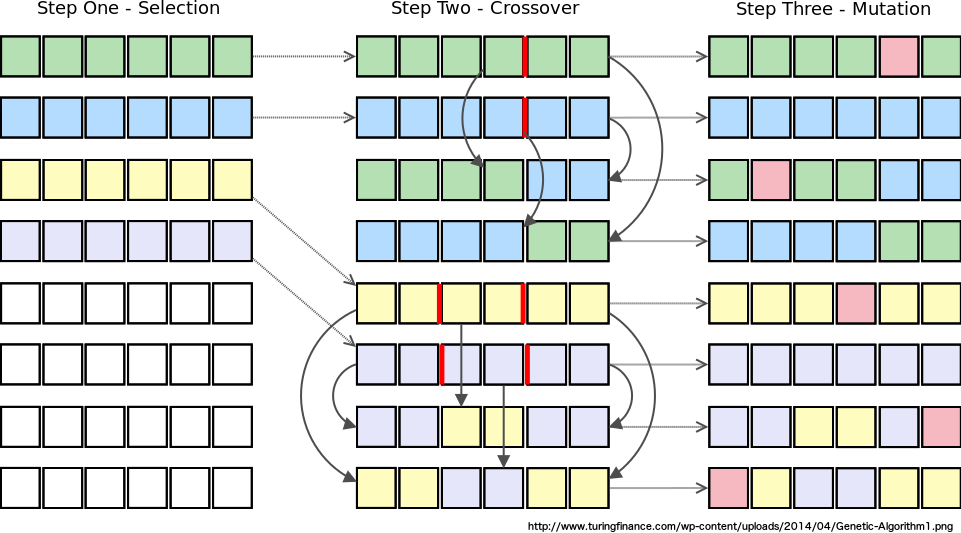
\includegraphics[width=1.0\linewidth]{pic003}
\end{minipage}
\end{mdframed} 
 
\begin{mdframed}[backgroundcolor=white,roundcorner=4pt,shadow=true,linewidth=1pt]
\color{Black}
\section*{Proposed Solution}
The model proposed is based on Genetic Algorithms (GA). GA is applied over a set of MIDI events. It is an unsupervised system which takes digital WAVE sounds as input and generates simplified, stylized vector data as output. 
\end{mdframed} 
 
\begin{mdframed}[backgroundcolor=white,roundcorner=4pt,shadow=true,linewidth=1pt]
\color{Black}
\section*{Sound Simplification}
A WAVE sound usually contains details that are not relevant for the audio quality and increase the cost of computations. Simplification of WAVE sounds is a process to eliminate the most useless elements, while retaining the perceptually dominant elements. Simplification of WAVE sound is used in the area of music composition and game development. In sounds simplification and vectorization digital WAVE samples are the input and generated simplified, stylized vector data are the output. The objective of sounds simplification by vectorization is to split the original sound into simple MIDI events. 
\end{mdframed} 
 
\begin{mdframed}[backgroundcolor=white,roundcorner=4pt,shadow=true,linewidth=1pt]
\color{Black}
\section*{Solution Encoding}
In this study MIDI events were chosen as approximation primitives to be used for sound reconstruction. Each MIDI event is described by its type, status and time. Each individual in the GA's population consists of an ordered set of events and a fitness value. 
\end{mdframed} 
 
\begin{mdframed}[backgroundcolor=white,roundcorner=4pt,shadow=true,linewidth=1pt]
\color{Black}
\section*{Fitness Value}
The fitness value is calculated as Euclidean distance between the approximate sound and the original sound. The approximated sound is assembled by MIDI events. 
\end{mdframed} 
 
\begin{mdframed}[backgroundcolor=white,roundcorner=4pt,shadow=true,linewidth=1pt]
\color{Black}
\section*{Initial Population}
As an initial step GA population is initialized with randomly generated sets of events. Type, status and time are taken randomly for each event. 
\end{mdframed} 
 
\begin{mdframed}[backgroundcolor=white,roundcorner=4pt,shadow=true,linewidth=1pt]
\color{Black}
\section*{Optimization Parameters}
During GA's evolutionary process individuals are selected from the population, crossover, mutation, evaluation and survival are applied so that the sound approximation is approved. In this study a binary crossover is chosen. Mutation is applied as time shifting and status change of one event in the individual. During evaluation phase the approximated sound is compared with the original sound. The result of the comparison is used as a fitness value of the individual. During the survival process it is decided which individual to be kept, the newly created or the already existing. The only stopping criteria used is the total number of sound evaluations.
\end{mdframed}

% Заключение.
\begin{mdframed}[backgroundcolor=white,roundcorner=4pt,shadow=true,linewidth=1pt]
\color{Black}
\section*{Conclustions}
Experiments show that using GA may be very efficient and sound approximation is relatively accurate in the limits of the sound simplification. Optimization convergence is related to the probabilistic nature of GA. Sound comparison is time consuming and slows down the optimization process. As further research, it could be suitable for GA to be implemented as distributed computing algorithm. Such a distributed implementation is efficiently applicable for the class of evolutionary algorithms GA is a part of. The set of events can be treated as a multidimensional space and optimization can provide much better results.
\end{mdframed}

% Секция за служебна информация.
\begin{mdframed}[backgroundcolor=white,roundcorner=4pt,shadow=true,linewidth=1pt]
\color{Black}

% Биглиография.
\section*{References}
\begin{enumerate}
\item T. Balabanov, M. Barova, D. Keremedchiev, \textit{Image Construction with 2D Ellipses by Genetic Algorithms Optimization}, 11th Annual Meeting of the Bulgarian Section of SIAM, 2016.
\item G. Evtimov, D. Keremedchiev, M. Barova, \textit{Image Vectorization and Colors Reduction with Ant Colony Optimization}, Advances in Mathematics: Scientific Journal, 2016.
\item T. Balabanov, \textit{Distributed Evolutional Model for Music Composition by Human-Computer Interaction}, International Scientific Conference UniTech, 2015.
\item R. Johansson, \textit{Genetic Programming: Evolution of Mona Lisa}, .NET, Go, Distributed Programming, 2008.
\item T. Balabanov, \textit{Distributed System for Automated Generation of Music Melodies Through Human-Computer Interaction} (in Bulgarian), MSc Thesis at NBU, Sofia, Bulgaria, 2008.
\end{enumerate}
\end{mdframed}

% Благодарности.
\begin{mdframed}[backgroundcolor=white,roundcorner=4pt,shadow=true,linewidth=1pt]
\section*{Acknowledgements}
This work was supported by a private funding of Velbazhd Software LLC. 


\includegraphics[width=1.0\linewidth]{veld_soft_camp_fire_logo}
\end{mdframed}
\end{multicols}

% Информация за конференцията. 
\begin{mdframed}[backgroundcolor=white,roundcorner=4pt,shadow=true,linewidth=1pt]
\color{Black}
12th Annual Meeting of the Bulgarian Section of SIAM, December 20 - 22, 2017, Sofia, Bulgaria
\end{mdframed}

\end{document}
